\documentclass{article}

\usepackage{graphicx}

\begin{document}

\section{Virtual function implementation}

\begin{verbatim}
struct B {
  ...
  virtual int vf0();
  virtual int vf1();
  ...
  virtual int vf4();
};
\end{verbatim}
{\tt {B}} layout becomes like figure \ref{derived_e000}.

\vspace{0.5cm}
\begin{figure}[htbp]
\begin{center}
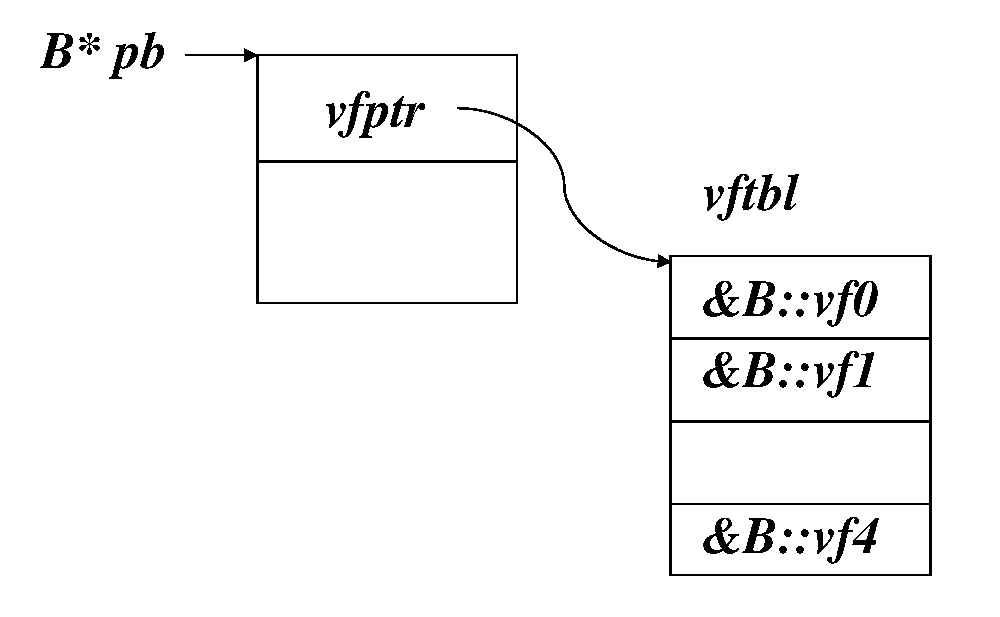
\includegraphics[width=1.0\linewidth,height=0.6\linewidth]{virtual_function.eps}
\caption{{\tt{B}} layout}
\label{derived_e000}
\end{center}
\end{figure}

So, for virtual function call like
\begin{verbatim}
int g(B* pb){ return pb->vf3(); }
\end{verbatim}
3 address code for this becomes like bellow:
\begin{verbatim}
g:
  t0 := *pb
  t1 := t0 + (offset of positon &B:vf3 at vftbl)
  t2 := *t1
  t3 := call t2
  return t3
\end{verbatim}

If {\tt{D}} is derived from {\tt{B}} like bellow:
\begin{verbatim}
struct D : B {
  int vf3();  // Override vf3
  virtual int vf5();
  virtual int vf6();
  ...
  virtual int vf9();
};
\end{verbatim}
{\tt {D}} layout becomes like figure \ref{derived_e002}.

\vspace{0.5cm}
\begin{figure}[htbp]
\begin{center}
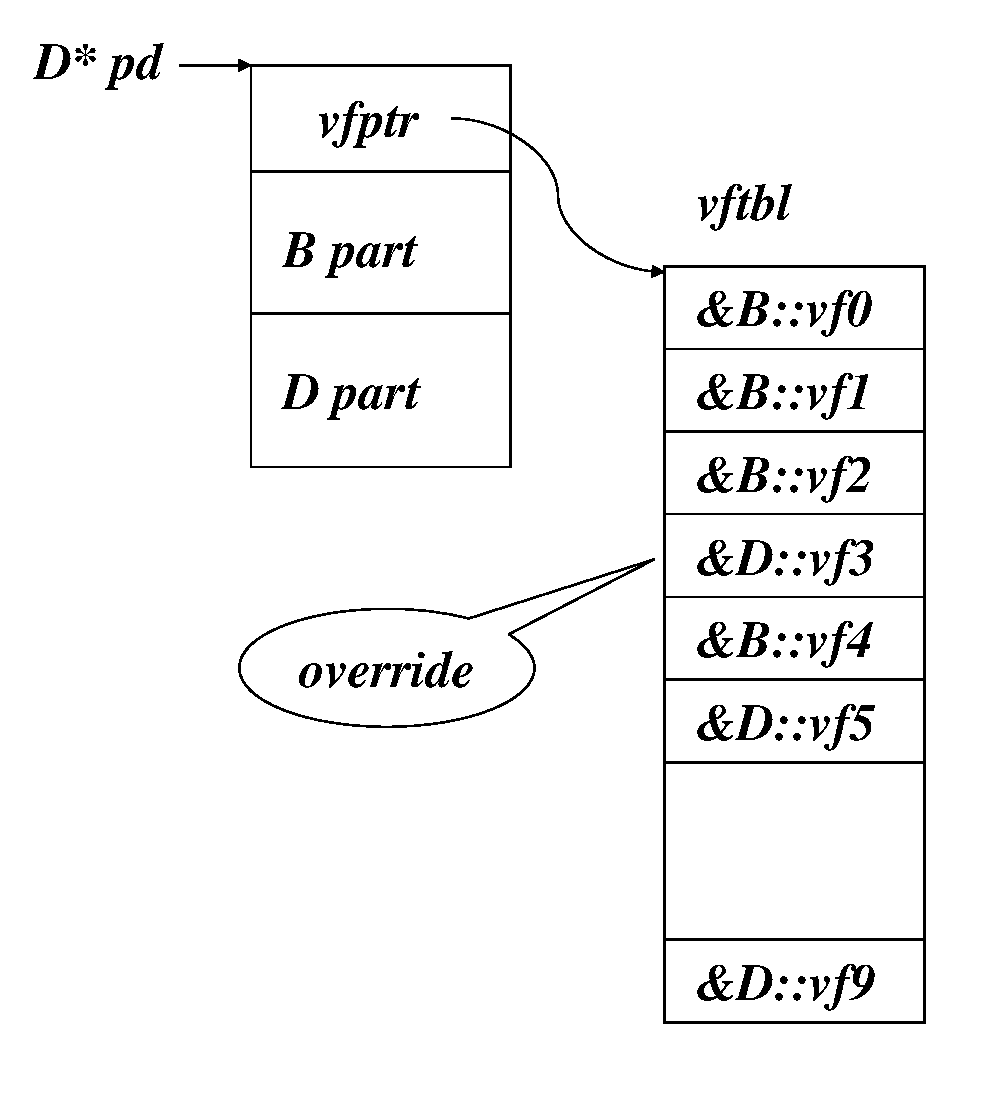
\includegraphics[width=0.91\linewidth,height=1.0\linewidth]{virtual_function2.eps}
\caption{{\tt{D}} layout}
\label{derived_e002}
\end{center}
\end{figure}

\section{Virtual base implementation}

\begin{verbatim}
struct B0 { /* ... */ };
struct B1 { /* ... */ };
...
struct B4 { /* ... */ };
struct D : virtual B0, virtual B1, ..., virtual B4 {};
\end{verbatim}
{\tt {D}} layout becomes like figure \ref{derived_e001}.

\vspace{0.5cm}
\begin{figure}[htbp]
\begin{center}
\includegraphics[width=0.95\linewidth,height=1.0\linewidth]{virtual_base.eps}
\caption{{\tt{D}} layout}
\label{derived_e001}
\end{center}
\end{figure}

So,
\begin{verbatim}
B3* f(D* pd){ return (B3*)pd; }
\end{verbatim}
for the above code, 3 address code becomes like bellow:
\begin{verbatim}
f:
  t0 := *pd
  t1 := t0 + (offset of position delta B3 at vbtbl)
  t2 := *t1
  t3 := pd + t2
  return t3
\end{verbatim}

Unfortunately, the discussion is ended at this point. No discussion that
how {\tt{vbtbl}} is override. And no discussion that {\tt{(B3*)pd}}
is equivalent to {\tt{static\_cast<B3*>(pd)}} or other version cast.  
\end{document}

